%!TEX root = main.tex

\subsection{Simple Genome Statistics}

\subsubsection{GC-content}

\textbf{GC-content} is the percentage of G or C in a DNA sequence.


\begin{figure}[htp]
	\centering
	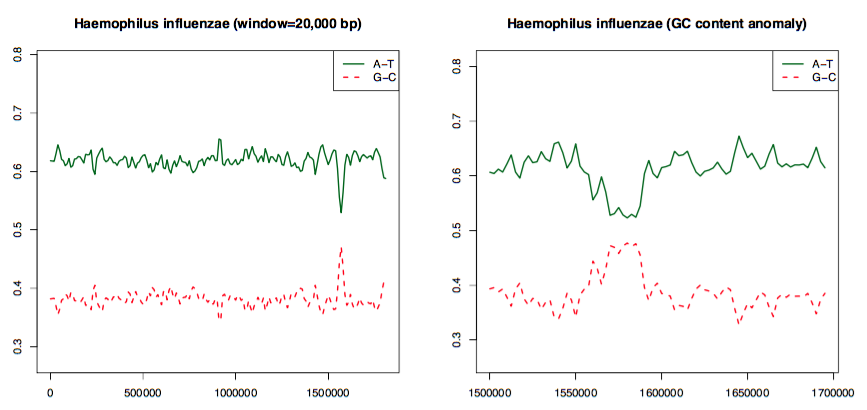
\includegraphics[scale=0.4]{images/01_gc.png}
 	\caption{GC-Content. Anomaly due to an ancient insertion of viral DNA. AT-rich regions denature at lower temperature. The ability to quickly denature DNA facilitates the insertion in the bacterial cell being infected.}
\end{figure}

\subsubsection{Dimer frequencies}

Some dimers are particulary frequent but it is due to have each nitrogenous bases frequent. Need a background model.

\begin{figure}[htp]
	\centering
	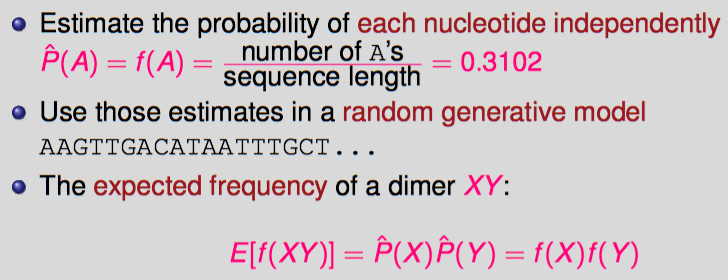
\includegraphics[scale=0.4]{images/02_dimer.png}
 	\caption{Multinomial background model.}
\end{figure}

With the multinomial background model, we can compute the \textbf{odd ratios}: ratio between observed frequency and expected frequency: $\frac{f(XY)}{E[f(XY)]} = \frac{f(XY)}{f(X)f(Y)}$.


The multinomial model is  equivalent to a random permutation of the original sequence: $\frac{f(XY)}{f_{random}(XY)}$.

We can generalize odd ratios to \textbf{k-mers}.

\begin{figure}[htp]
	\centering
	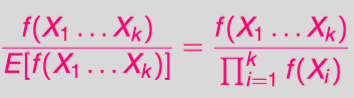
\includegraphics[scale=0.4]{images/03_kmers.png}
 	\caption{k-mers. Useful when looking for frequent patterns of k consecutive characters. But are they informative ? Need a more sophisticated background model, a statistical test to assess signifiance and biological validation.}
\end{figure}

\subsection{Open Reading Frames}

\begin{figure}[htp]
	\centering
	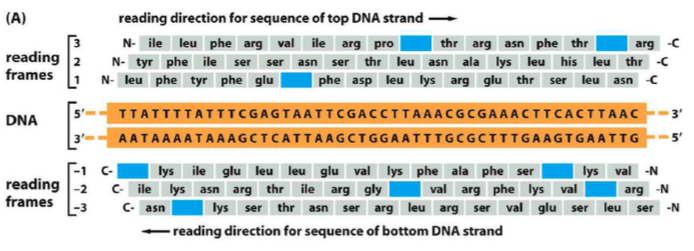
\includegraphics[scale=0.6]{images/04_rf.png}
 	\caption{Reading frames.}
\end{figure}

\subsubsection{Algorithm to find ORF}

\begin{figure}[H]
	\centering
	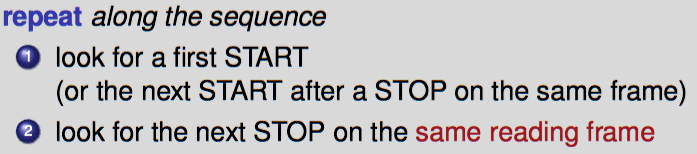
\includegraphics[scale=0.4]{images/05_algo.png}
 	\caption{Need to consider each reading frames (6). After a START, you may find other codons for Met before a STOP: not true START.   An ORF is a longest strech of DNA between a START and a STOP, without being interrupted by another STOP on the same frame.}
\end{figure}

The problem is to have to be sure that the ORF is a coding gene.
\begin{itemize}
	\item The DNA found between STAT and STOP codon might be due to chance: need \textbf{a statistical test procedure};
	\item The ORF might be there but the gene not expressed (trace of past or regulations at transcription/translation levels): need biological validation;
	\item Some gene sequences do not strictly follow the standard ORF structure: need biological validation.
\end{itemize}

\subsubsection{Signifiance assessment}

\begin{figure}[htp]
	\centering
	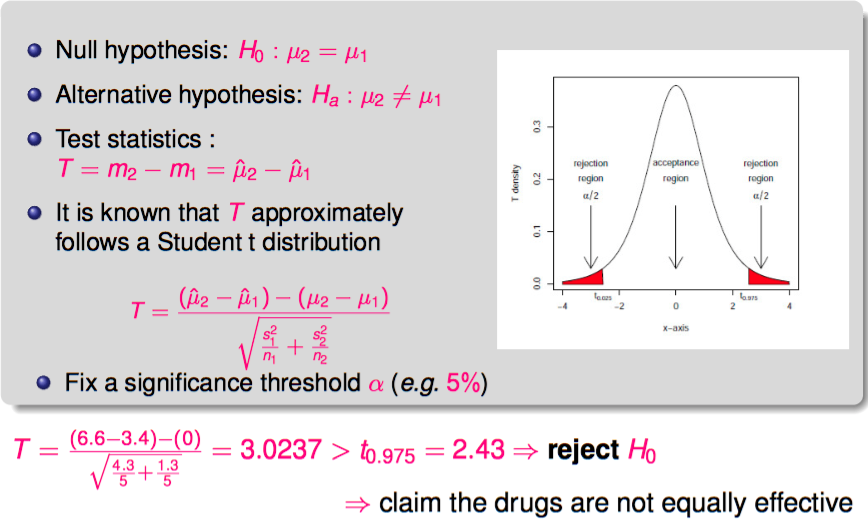
\includegraphics[scale=0.4]{images/06_test.png}
 	\caption{Statistical test. }
\end{figure}

To avoid fixing a signifiance threshold $\alpha$ we can compute the \textbf{p-value} of the test.

\begin{figure}[htp]
	\centering
	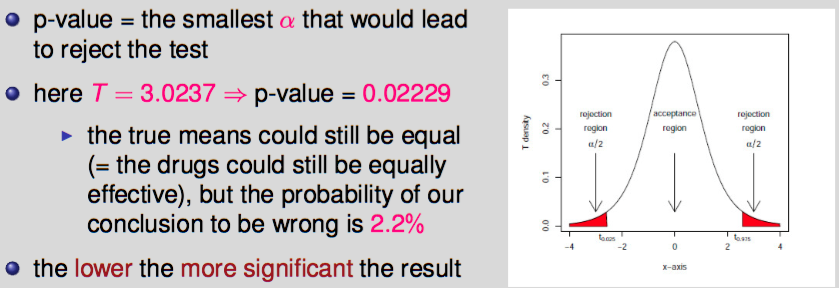
\includegraphics[scale=0.4]{images/07_pval.png}
 	\caption{p-value. }
\end{figure}

We can apply this to ORF.


\begin{figure}[htp]
	\centering
	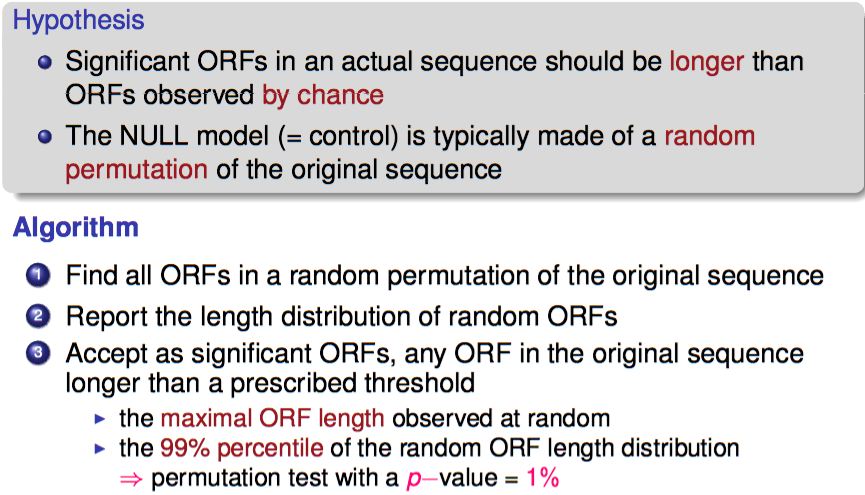
\includegraphics[scale=0.4]{images/08_orf.png}
 	\caption{Algorithm to assess signifiance of ORF.}
\end{figure}